% -*- latex -*-
%%%%%%%%%%%%%%%%%%%%%%%%%%%%%%%%%%%%%%%%%%%%%%%%%%%%%%%%%%%%%%%%
%%%%%%%%%%%%%%%%%%%%%%%%%%%%%%%%%%%%%%%%%%%%%%%%%%%%%%%%%%%%%%%%
%%%%
%%%% This text file is part of the lecture slides for
%%%% `Parallel Computing'
%%%% by Victor Eijkhout, copyright 2012-2020
%%%%
%%%% Onesided-slides.tex : slides about one-sided communication
%%%%
%%%%%%%%%%%%%%%%%%%%%%%%%%%%%%%%%%%%%%%%%%%%%%%%%%%%%%%%%%%%%%%%
%%%%%%%%%%%%%%%%%%%%%%%%%%%%%%%%%%%%%%%%%%%%%%%%%%%%%%%%%%%%%%%%

\begin{numberedframe}{Overview}
  This section concernes one-sided operations, which allows `shared
  memory' type programming. (Actual shared memory later.)

  Commands learned:
  \begin{itemize}
  \item \indexmpishow{MPI_Put}, \indexmpishow{MPI_Get}, \indexmpishow{MPI_Accumulate}
  \item Window commands: \indexmpishow{MPI_Win_create}, \indexmpishow{MPI_Win_allocate}
  \item Active target synchronization \indexmpishow{MPI_Win_fence}
  \item \indexmpishow{MPI_Win_post}\lstinline{/wait/start/complete}
  \item Passive target synchronization \indexmpishow{MPI_Win_lock}~/
    \indexmpishow{MPI_Win_lock}
  \item Atomic operations: \indexmpishow{MPI_Fetch_and_op}
  \end{itemize}
\end{numberedframe}

\sectionframe{Basic mechanisms}

\begin{numberedframe}{Motivation}
  With two-sided messaging, you can not just put data
  on a different processor: the other has to expect it and receive it.

  \begin{itemize}
  \item Sparse matrix: it is easy to know what you are receiving, not
    what you need to send.  Usually solved with complicated
    preprocessing step.
  \item Neuron simulation: spiking neuron propagates information to neighbours.
    Uncertain when this happens.
  \item Other irregular data structures: distributed hash tables.
  \end{itemize}
\end{numberedframe}

\begin{numberedframe}{Dynamic data}
\begin{lstlisting}
x = f();
p = hash(x);
MPI_Send( x, /* to: */ p );
\end{lstlisting}
Problem: how does \lstinline{p} know to post a receive,\\
and how does everyone else know not to?
\end{numberedframe}

\begin{numberedframe}{One-sided concepts}
  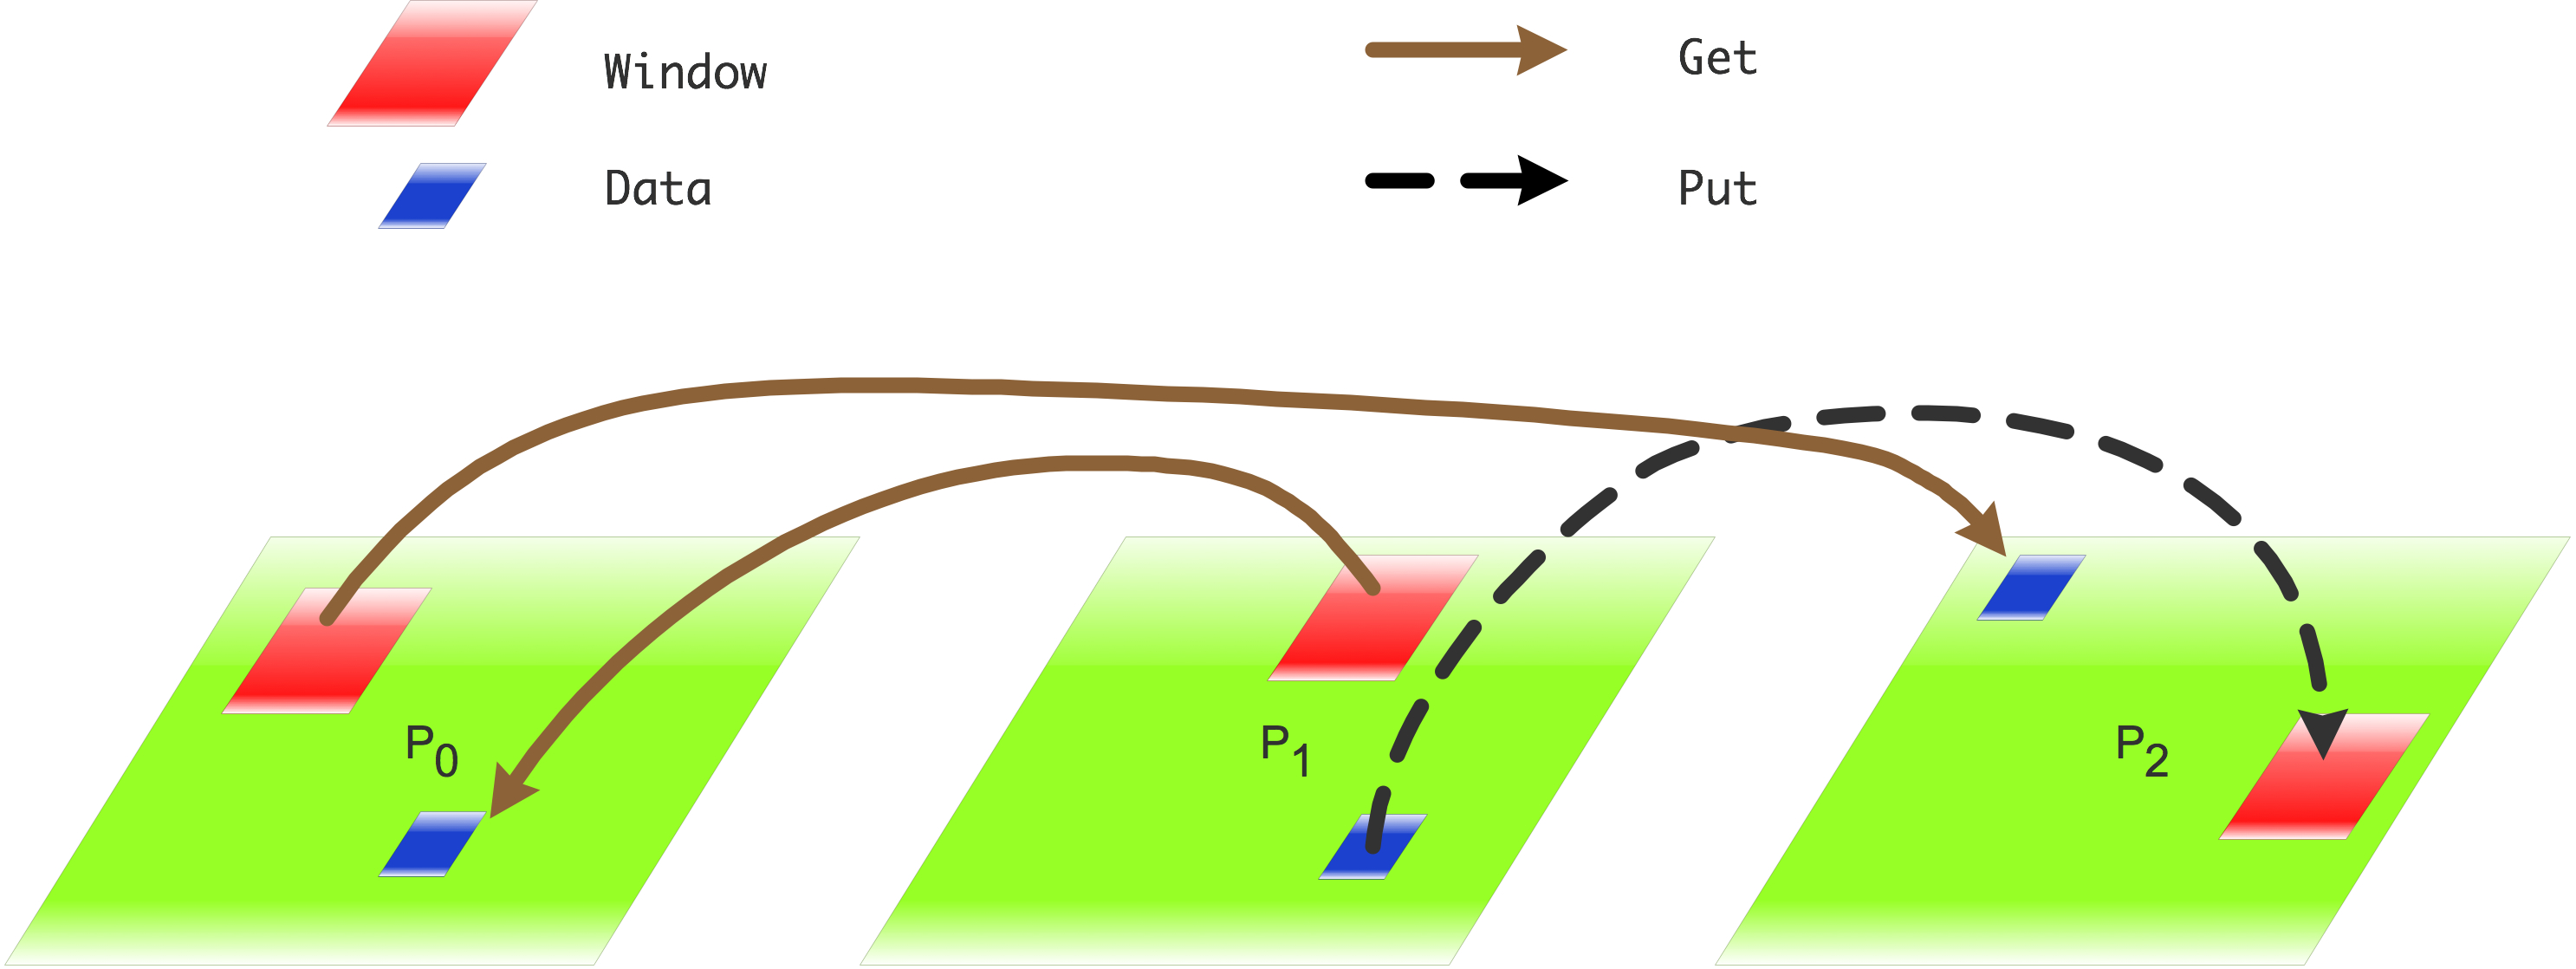
\includegraphics[scale=.1]{one-sided-getput}
  \begin{itemize}
  \item A process has a \indexterm{window} that other processes can access.
  \item \indexterm{origin}: process doing a one-sided call\\
    \indexterm{target}: process being accessed.
  \item One-sided calls: \indexmpishow{MPI_Put}, \indexmpishow{MPI_Get}, \indexmpishow{MPI_Accumulate}.
  \item Various synchronization mechanisms.
  \end{itemize}
\end{numberedframe}

\begin{numberedframe}{Window creation}
  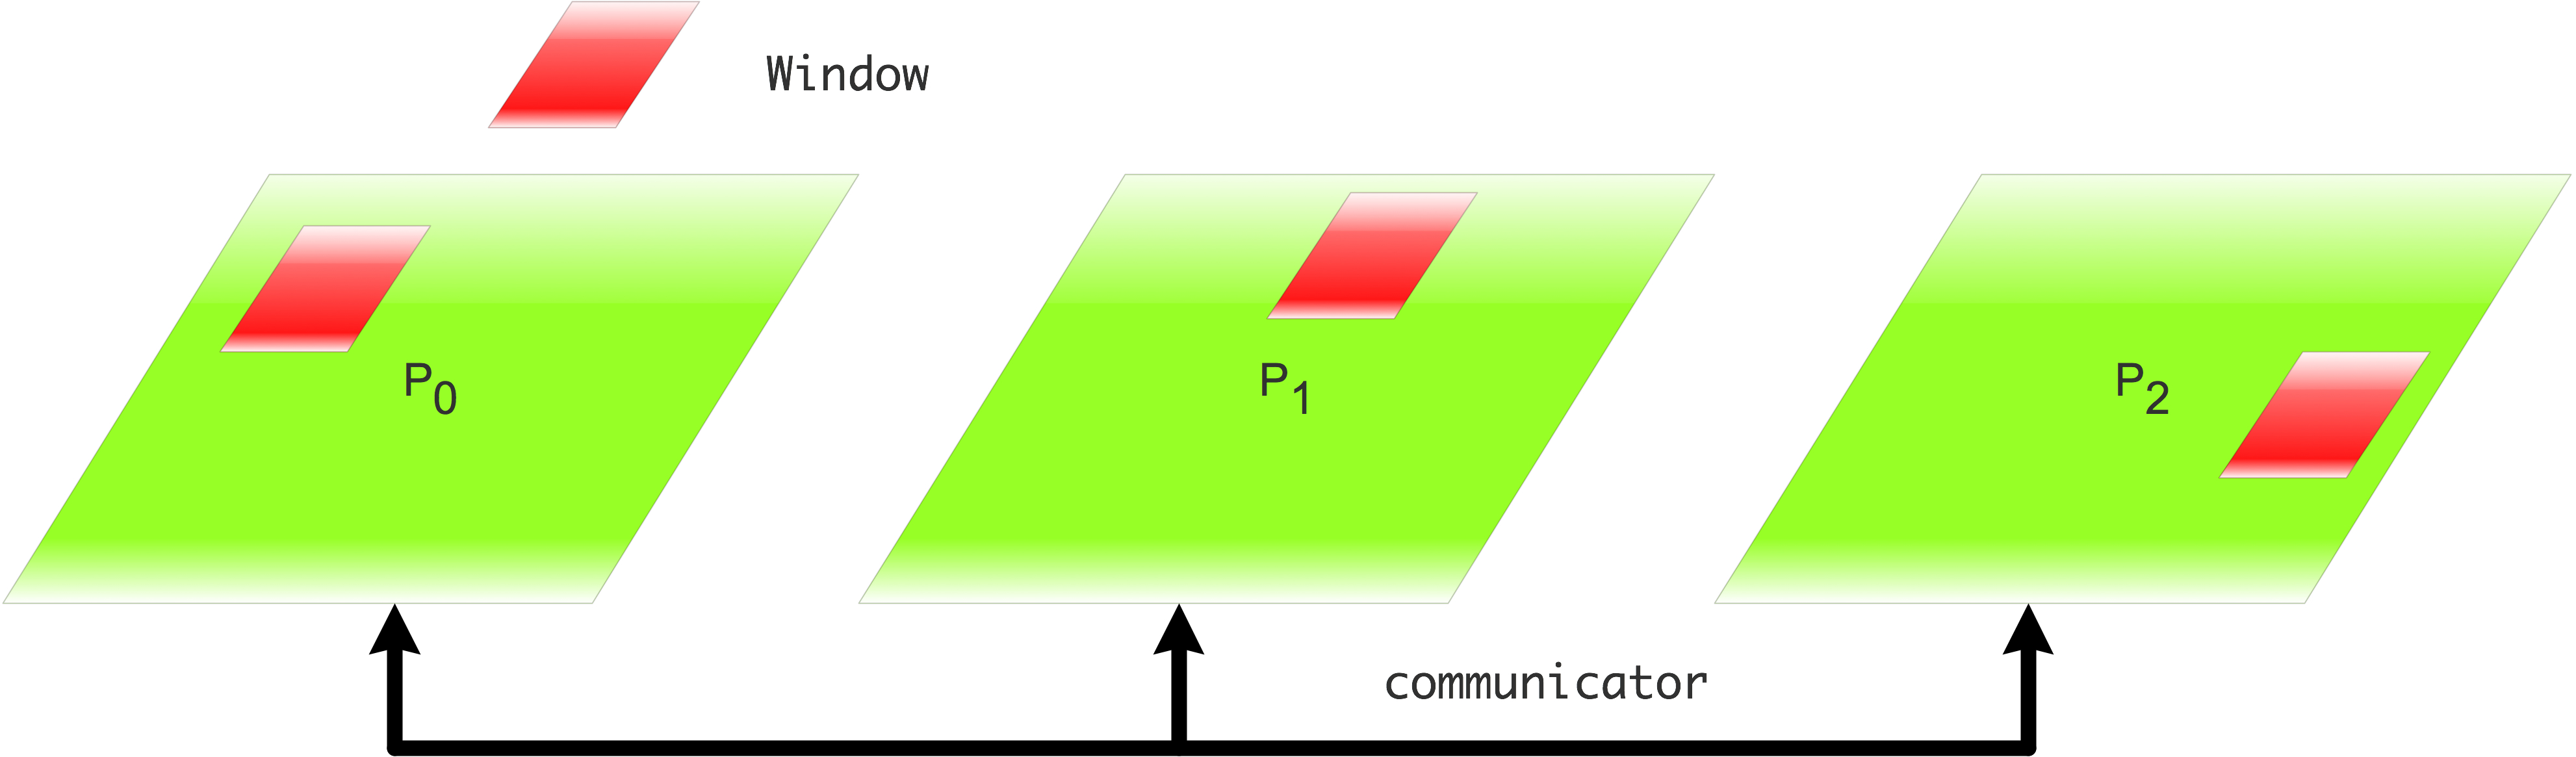
\includegraphics[scale=.08]{one-sided-window}
\lstset{language=C}
\begin{lstlisting}
MPI_Win_create (void *base, MPI_Aint size, 
  int disp_unit, MPI_Info info, MPI_Comm comm, MPI_Win *win)
\end{lstlisting}
\begin{itemize}
\item \lstinline{size}: in bytes
\item \lstinline{disp_unit}: \lstinline{sizeof(type)}
\end{itemize}
Also call \indexmpishow{MPI_Win_free} when done. This is important!
\end{numberedframe}

\begin{numberedframe}{Window allocation}
  Instead of passing buffer, let MPI allocate with
  \indexmpishow{MPI_Win_allocate}\\
  and return the buffer pointer:
\lstset{language=C}
\begin{lstlisting}
int MPI_Win_allocate
   (MPI_Aint size, int disp_unit, MPI_Info info,
    MPI_Comm comm, void *baseptr, MPI_Win *win)
\end{lstlisting}
can use dedicated fast memory.
\end{numberedframe}

\begin{numberedframe}{Active target synchronization}
  All processes call \indexmpishow{MPI_Win_fence}. Epoch is between fences:
\lstset{language=C}
\begin{lstlisting}
MPI_Win_fence(MPI_MODE_NOPRECEDE, win);
if (procno==producer)
  MPI_Put( /* operands */, win);
MPI_Win_fence(MPI_MODE_NOSUCCEED, win);
\end{lstlisting}
Second fence indicates that one-sided communication is concluded:\\
target knows that data has been put.
\end{numberedframe}

\protoslide{MPI_Put}

\begin{numberedframe}{Location in the window}
  Location to write:
  \[ \mathtt{window\_base} + \mathtt{target\_disp}\times \mathtt{disp\_unit}. \]
  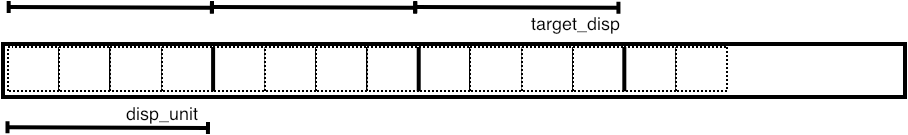
\includegraphics[scale=.4]{windowdisp}
\end{numberedframe}

\begin{exerciseframe}[rightput]
  \input ex:rightput
\end{exerciseframe}

\begin{exerciseframe}[randomput]
  \input ex:randomput
\end{exerciseframe}

\begin{optexerciseframe}[randomput]
  Replace \indexmpishow{MPI_Win_create} by \indexmpishow{MPI_Win_allocate}.
\end{optexerciseframe}

\begin{numberedframe}{Remaining simple routines:
    Get, Accumulate}
  \begin{itemize}
  \item \indexmpishow{MPI_Get} is converse of \indexmpishow{MPI_Put}. Like Recv, but no
    status argument.
  \item \indexmpishow{MPI_Accumulate} is a Put plus a reduction on the result:
    multiple accumulate calls in one epoch well-defined.\\
    Can use any predefined \indexmpishow{MPI_Op} (not user-defined) or \indexmpishow{MPI_REPLACE}.
  \end{itemize}
\end{numberedframe}



\protoslide{MPI_Get}
\protoslide{MPI_Accumulate}

\sectionframe{Ordering and synchronization}

\begin{numberedframe}{Fence synchronization}
  Already mentioned active target synchronization:\\
  the target indicates the start/end of an epoch.

  Simplest mechanism: \indexmpishow{MPI_Win_fence}, collective.  

  After the closing fence, buffers have been sent~/ windows have been updated.
\end{numberedframe}

\begin{numberedframe}{Ordering of operations}
  Ordering is often undefined:
  \begin{itemize}
  \item No ordering of Get and Put/Accumulate operations
  \item No ordering of multiple Puts. Use Accumulate.
  \end{itemize}
  The following operations are well-defined inside one epoch:
  \begin{itemize}
  \item Instead of multiple Put operations, use Accumulate with
    \indexmpishow{MPI_REPLACE}.
  \item \indexmpishow{MPI_Get_accumulate} with
    \indexmpishow{MPI_NO_OP} is safe.
  \item Multiple Accumulate operations from one origin are ordered by
    default.
  \end{itemize} 
\end{numberedframe}

\begin{optexerciseframe}[countdown]
  \input ex:countdown
\end{optexerciseframe}

\begin{numberedframe}{A second active synchronization}
  Use \indexmpishow{MPI_Win_post}, \indexmpishow{MPI_Win_wait},
  \indexmpishow{MPI_Win_start}, \indexmpishow{MPI_Win_complete} calls

  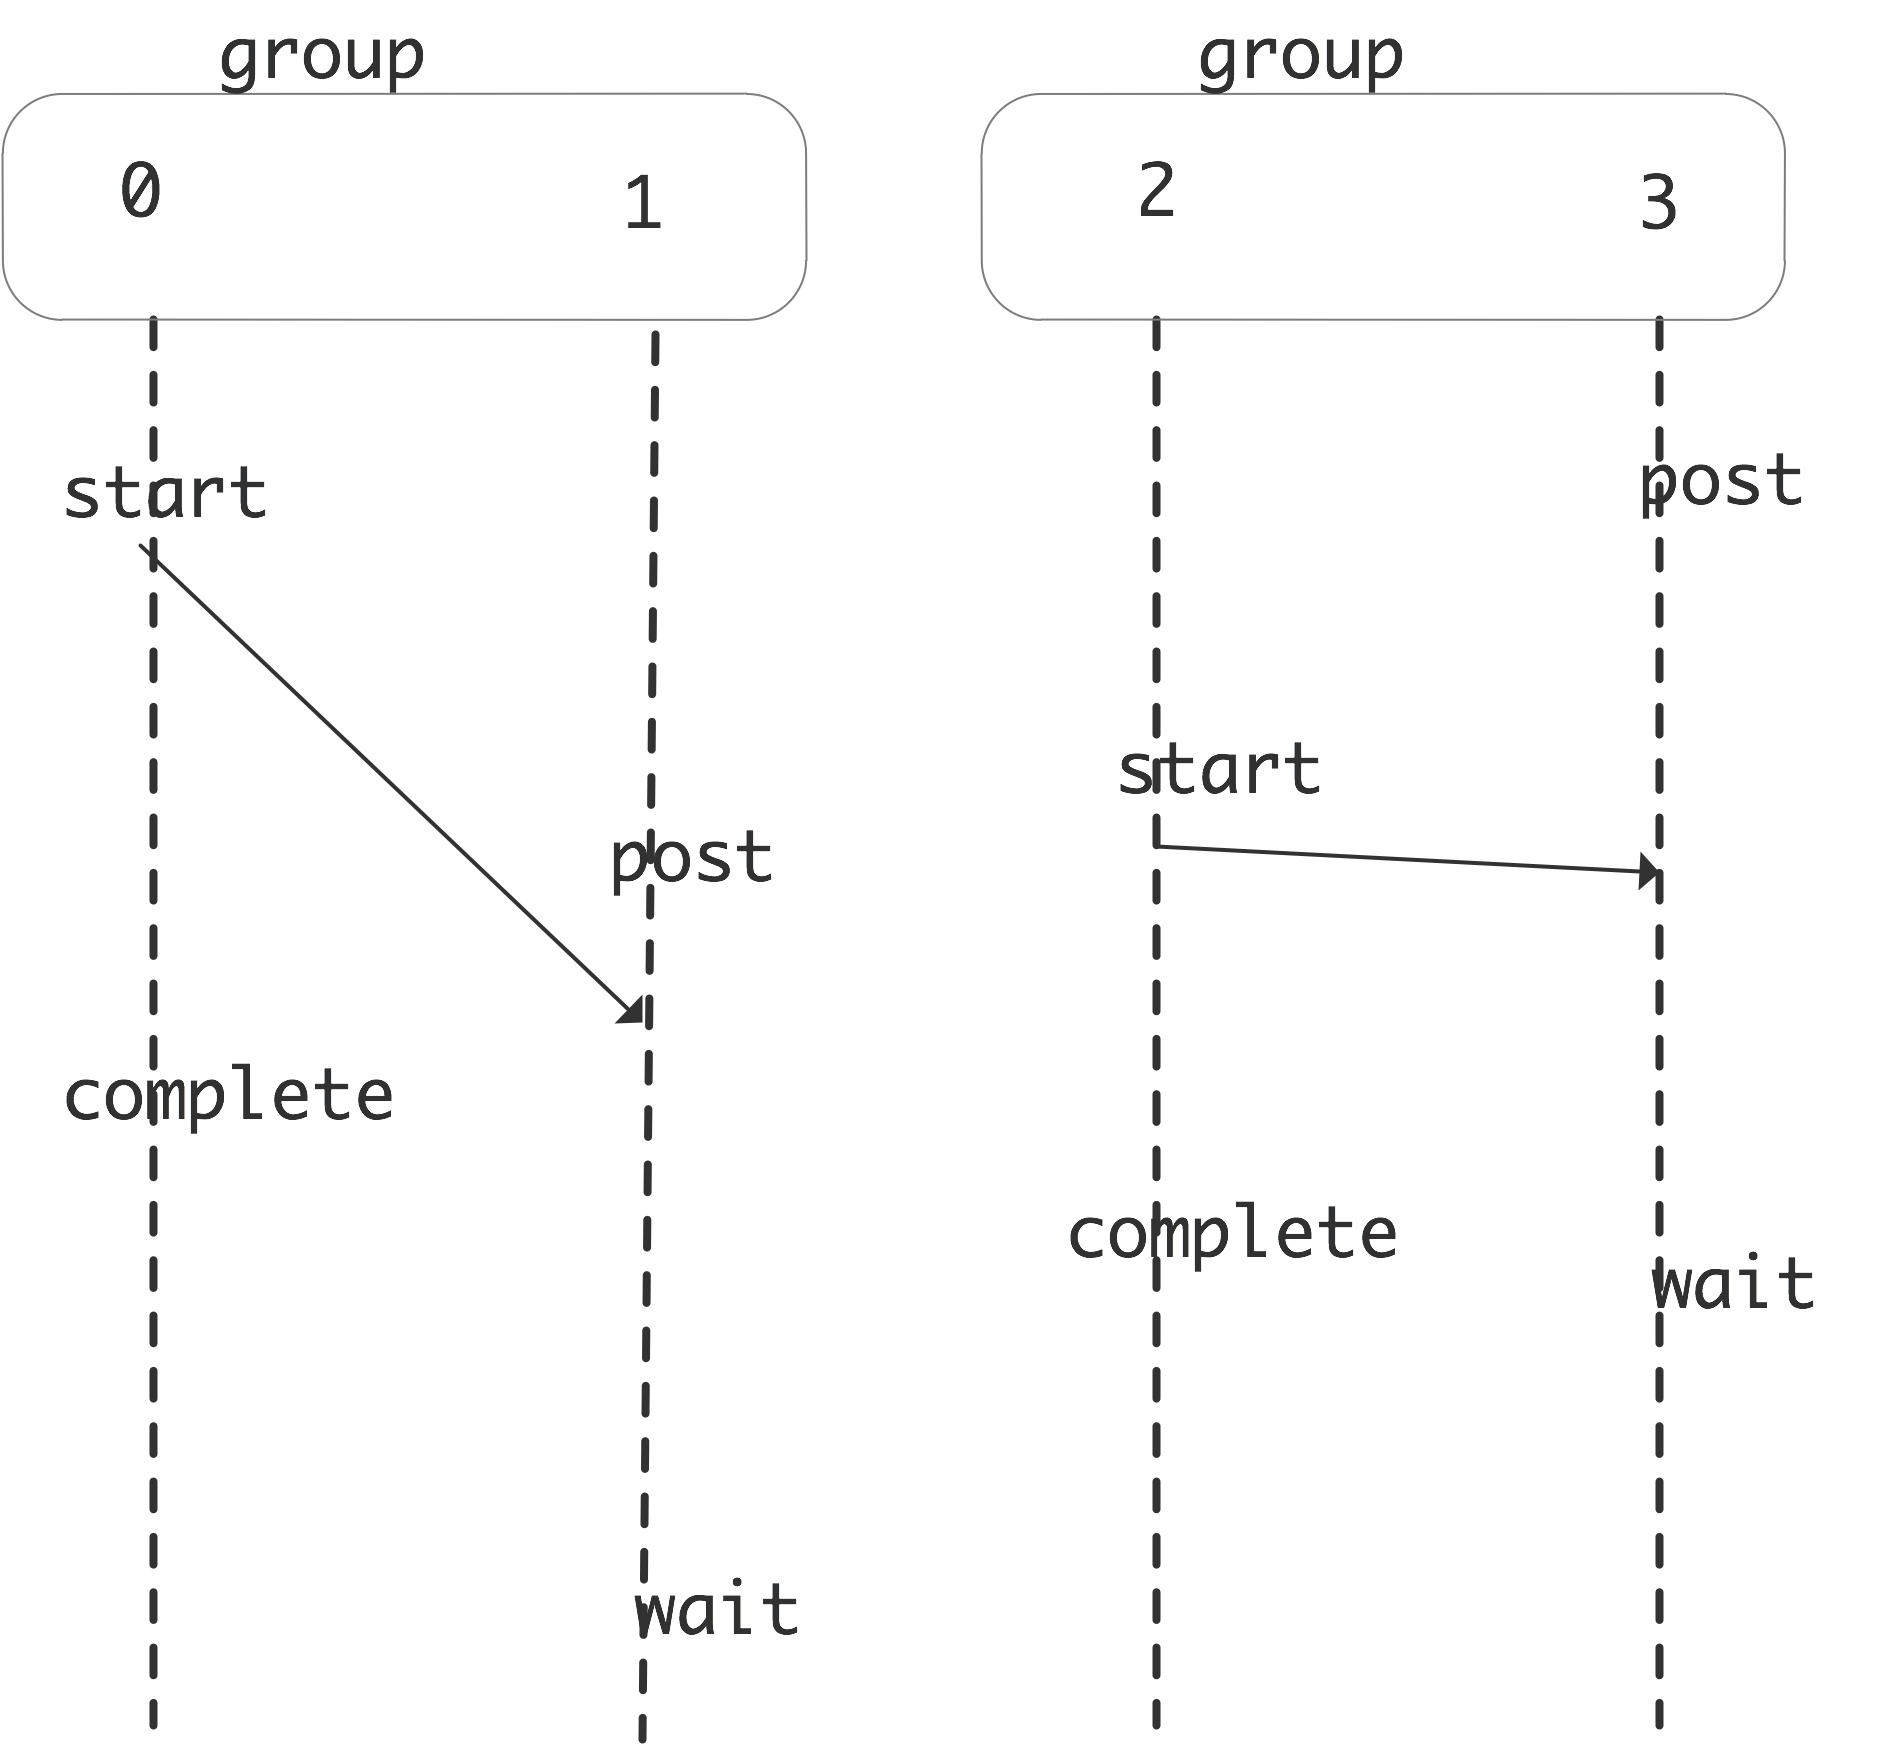
\includegraphics[scale=.1]{postwait}

  More fine-grained than fences.
\end{numberedframe}

\sectionframe{Passive target synchronization}

\begin{numberedframe}{Passive target synchronization}
  Lock a window on the target:
\lstset{language=C}
\begin{lstlisting}
MPI_Win_lock
   (int locktype, int rank, int assert, MPI_Win win)
MPI_Win_unlock
   (int rank, MPI_Win win)
\end{lstlisting}
  with types:  \indexmpishow{MPI_LOCK_SHARED} \indexmpishow{MPI_LOCK_EXCLUSIVE}
\end{numberedframe}

\endinput

\begin{numberedframe}{}
\begin{lstlisting}
  
\end{lstlisting}
\end{numberedframe}

